% !TEX root = ../enac_project_fr.tex
%%%%%%%%%%%%%%%%%%%%%%%%%%%%%%%%%%%%%%%%%%%%%%%%%%%%%%%%%%%%%%%%%%%%
% Chapter 3 - Passage en Precise Point Positioning
%%%%%%%%%%%%%%%%%%%%%%%%%%%%%%%%%%%%%%%%%%%%%%%%%%%%%%%%%%%%%%%%%%%%

\chapter{Passage en Precise Point Positioning (PPP)}
\label{precise_point_positioning}

La chaîne décrite au chapitre~\ref{chaine_traitement_positionnement_gnss}
utilise des observations GNSS non différenciées et estime la position d'un
récepteur unique. Elle possède donc déjà la structure générale d'un
positionnement ponctuel. Sa précision reste toutefois limitée par les
éphémérides et les horloges diffusées, ainsi que par les biais instrumentaux
qui ne peuvent plus être négligés lorsque l'objectif devient centimétrique.

Le passage au \textit{Precise Point Positioning} (PPP) consiste à remplacer
les orbites et horloges diffusées par des produits précis issus d'un réseau
mondial de stations, puis à rendre le modèle d'observation cohérent avec ces
produits. Il ne nécessite aucune station de référence à proximité du
récepteur. Dans le cadre de cette étude, cette évolution permet d'atteindre
une erreur tridimensionnelle d'environ $1\,\mathrm{cm}$ en fin de convergence.
Une telle précision constitue également une base adaptée à de futurs travaux
de détermination précise d'orbite (POD), qui ne sont pas développés ici.

\section{Principe du Precise Point Positioning}

Le PPP exploite conjointement les pseudo-distances et les phases de porteuse,
généralement sur deux fréquences. Les observations restent non différenciées :
les erreurs communes ne sont pas éliminées par différence entre stations ou
satellites, mais corrigées par des modèles ou estimées comme paramètres.

Pour un satellite $s$ et un récepteur $r$, les observations corrigées sur la
fréquence $i$ s'écrivent, en mètres,

\begin{align}
P_{r,i}^{s}
&=
\rho_r^s
+c\left(\delta t_r-\delta t^s\right)
+T_r^s
+I_{r,i}^s
+\delta_{\mathrm{Sagnac},r}^s
+\delta_{\mathrm{Shapiro},r}^s
+\delta_{\mathrm{ant},r,i}
+\delta_{\mathrm{ant},i}^{s}
+b_{r,i}^{P}+b_i^{P,s}
+\varepsilon_{r,i}^{P,s},
\label{eq:ppp_code_raw}
\\
\begin{split}
L_{r,i}^{s}
&=
\rho_r^s
+c\left(\delta t_r-\delta t^s\right)
+T_r^s
-I_{r,i}^s
+\lambda_i N_{r,i}^{s}
+\delta_{\mathrm{Sagnac},r}^s
+\delta_{\mathrm{Shapiro},r}^s
\\
&\quad
+\delta_{\mathrm{ant},r,i}
+\delta_{\mathrm{ant},i}^{s}
+\delta_{\mathrm{wind\text{-}up},r,i}^s 
+b_{r,i}^{L}+b_i^{L,s}
+\varepsilon_{r,i}^{L,s}.
\end{split}
\label{eq:ppp_phase_raw}
\end{align}

avec :

\begin{itemize}
    \item $\rho_r^s = \|\mathbf{r}^s - \mathbf{r}_r\|$ la distance géométrique satellite-récepteur ;
    \item $\delta t_r$ et $\delta t^s$ les biais d'horloge du récepteur et du satellite ;
    \item $T_r^s$ le retard troposphérique ;
    \item $I_{r,i}^s$ le retard ionosphérique (avance apparente sur la phase, signe opposé) ;
    \item $\delta_{\mathrm{Sagnac},r}^s$ la correction de Sagnac, introduite au chapitre~\ref{sagnac} ;
    \item $\delta_{\mathrm{Shapiro},r}^s$ le retard de Shapiro, introduit au chapitre~\ref{shapiro} ;
    \item $\delta_{\mathrm{ant},r,i}$ et $\delta_{\mathrm{ant},i}^{s}$ les corrections de centre de phase (PCO, PCV) des antennes du récepteur et du satellite, détaillées en section~\ref{sec:antenna_corrections} ;
    \item $\delta_{\mathrm{wind\text{-}up},r,i}^s$ la correction d'enroulement de phase (phase uniquement), détaillée en section~\ref{windup} ;
    \item $b_{r,i}^{P}$, $b_i^{P,s}$, $b_{r,i}^{L}$, $b_i^{L,s}$ les biais instrumentaux (OSB) de code et de phase du récepteur et du satellite présentés en section~\ref{biais_obs} ;
    \item $N_{r,i}^s$ l'ambiguïté entière de phase, en cycles ;
    \item $\lambda_i = c/f_i$ la longueur d'onde de la fréquence $i$ ;
    \item $\varepsilon_{r,i}^{P,s}$ et $\varepsilon_{r,i}^{L,s}$ les erreurs résiduelles de code et de phase.
\end{itemize}

La combinaison ionosphère-libre présentée au chapitre précédent est retenue
afin d'éliminer le terme ionosphérique du premier ordre. Pour deux fréquences
$f_1$ et $f_2$, ses coefficients sont

\begin{align}
\alpha=\frac{f_1^2}{f_1^2-f_2^2},
\qquad
\beta=-\frac{f_2^2}{f_1^2-f_2^2},
\qquad
\alpha+\beta=1.
\label{eq:ppp_if_coefficients}
\end{align}

Après correction des biais propres à chaque observable, les combinaisons de
code et de phase sont

\begin{align}
P_{r,\mathrm{IF}}^s
&=\alpha P_{r,1}^{s,\mathrm{corr}}
+\beta P_{r,2}^{s,\mathrm{corr}},
\\
L_{r,\mathrm{IF}}^s
&=\alpha L_{r,1}^{s,\mathrm{corr}}
+\beta L_{r,2}^{s,\mathrm{corr}}.
\label{eq:ppp_if_observations}
\end{align}

Le modèle PPP ionosphère-libre devient alors

\begin{align}
P_{r,\mathrm{IF}}^s
&=\rho_r^s
+c\left(\delta t_r-\delta t^s_{\mathrm{prec}}\right)
+T_r^s
+\delta_{\mathrm{Sagnac},r}^s
+\delta_{\mathrm{Shapiro},r}^s
+\delta_{\mathrm{ant},r,\mathrm{IF}}
+\delta_{\mathrm{ant},\mathrm{IF}}^{s}
+\varepsilon_{r,\mathrm{IF}}^{P,s},
\label{eq:ppp_code_if}
\\
\begin{split}
L_{r,\mathrm{IF}}^s
&=\rho_r^s
+c\left(\delta t_r-\delta t^s_{\mathrm{prec}}\right)
+T_r^s
+\delta_{\mathrm{Sagnac},r}^s
+\delta_{\mathrm{Shapiro},r}^s
\\
&\quad
+\delta_{\mathrm{ant},r,\mathrm{IF}}
+\delta_{\mathrm{ant},\mathrm{IF}}^{s}
+\delta_{\mathrm{wind\text{-}up},r,\mathrm{IF}}^s
+B_{r,\mathrm{IF}}^s
+\varepsilon_{r,\mathrm{IF}}^{L,s}.
\end{split}
\label{eq:ppp_phase_if}
\end{align}

avec, pour les termes non encore introduits :

\begin{itemize}
    \item $\delta t^s_{\mathrm{prec}}$ le biais d'horloge précis du satellite, issu du produit CLK (section~\ref{sec:corrections_supplementaires}) ;
    \item $\delta_{\mathrm{ant},r,\mathrm{IF}}=\alpha\delta_{\mathrm{ant},r,1}+\beta\delta_{\mathrm{ant},r,2}$ la correction de centre de phase du récepteur combinée ionosphère-libre ;
    \item $\delta_{\mathrm{ant},\mathrm{IF}}^{s}=\alpha\delta_{\mathrm{ant},1}^{s}+\beta\delta_{\mathrm{ant},2}^{s}$ la correction de centre de phase du satellite combinée ionosphère-libre ;
    \item $\delta_{\mathrm{wind\text{-}up},r,\mathrm{IF}}^s=\alpha\delta_{\mathrm{wind\text{-}up},r,1}^s+\beta\delta_{\mathrm{wind\text{-}up},r,2}^s$ la correction d'enroulement de phase combinée ionosphère-libre ;
    \item $B_{r,\mathrm{IF}}^s$ l'ambiguïté ionosphère-libre, en mètres.
\end{itemize}

Contrairement à un positionnement par pseudo-distances époque par époque, le
PPP est un problème séquentiel. La position, l'horloge du récepteur, les
paramètres troposphériques et les ambiguïtés sont estimés conjointement. Un
vecteur d'état représentatif est

\begin{align}
\mathbf{x}
=
\begin{bmatrix}
\mathbf{r}_r^{\mathsf T} &
c\delta t_r &
Z_w &
G_N &
G_E &
B_1 & \cdots & B_m
\end{bmatrix}^{\mathsf T},
\label{eq:ppp_state}
\end{align}

où $Z_w$ est le retard troposphérique humide zénithal, $G_N$ et $G_E$ les
gradients horizontaux éventuels, et $B_1,\ldots,B_m$ les ambiguïtés des
satellites suivis. Selon le modèle retenu, la troposphère peut aussi être
entièrement corrigée par un modèle a priori, ou seul un retard zénithal peut
être estimé.

\section{Fichiers d'entrée pour le PPP}

Les fichiers RINEX d'observation restent la source des mesures de code, de
phase et de rapport signal sur bruit. Le fichier RINEX de navigation demeure
utile pour certaines informations auxiliaires et pour permettre un traitement
reposant sur les éphémérides diffusées. En mode PPP précis, les positions et
horloges satellites utilisées dans les équations~\eqref{eq:ppp_code_if} et
\eqref{eq:ppp_phase_if} proviennent toutefois des produits \texttt{SP3} et
\texttt{CLK}. Un produit \texttt{BIA} fournit les biais associés aux
observables. Ces trois fichiers doivent provenir d'une solution cohérente,
couvrir la période traitée et employer des conventions compatibles.

\subsection{Orbites précises SP3}

Un fichier \texttt{SP3} donne les coordonnées géocentriques des satellites à
des époques discrètes, éventuellement accompagnées de vitesses et
d'indicateurs de précision. Il remplace le calcul orbital fondé sur les
paramètres képlériens corrigés du message de navigation. La position à
l'instant d'émission $t_e$ est obtenue par interpolation :

\begin{align}
\mathbf{r}^s(t_e)
=
\mathcal{I}_{\mathrm{SP3}}
\!\left(t_e;\,\mathbf{r}^s_k\right),
\label{eq:sp3_interpolation}
\end{align}

où $\mathbf{r}^s_k$ désigne l'ensemble des points SP3 voisins. L'instant
d'émission dépend lui-même du temps de propagation $\tau$,

\begin{align}
t_e=t_r-\tau,
\qquad
\tau\simeq\frac{\rho_r^s}{c},
\label{eq:transmission_time}
\end{align}

ce qui impose une détermination cohérente de la géométrie à l'émission et à la
réception. Les transformations de repère doivent également tenir compte de la
rotation terrestre pendant la propagation du signal.

Les orbites précises sont généralement référencées au centre de masse du
satellite, tandis que les observations se rapportent au centre de phase de
son antenne. Le passage de l'un à l'autre nécessite le modèle d'attitude du
satellite et les corrections de centre de phase adaptées aux fréquences
utilisées.

\subsection{Horloges précises CLK}

Le fichier \texttt{CLK} contient les estimations précises du biais d'horloge
des satellites à des époques discrètes. À l'époque d'émission, la correction
utilisée est

\begin{align}
\delta t^s_{\mathrm{prec}}(t_e)
=
\mathcal{I}_{\mathrm{CLK}}
\!\left(t_e;\,\delta t^s_k\right).
\label{eq:clk_interpolation}
\end{align}

Une erreur temporelle $\Delta t$ produit directement une erreur de distance
$c\Delta t$ ; une précision centimétrique exige donc une connaissance de
l'horloge à quelques dizaines de picosecondes. Le produit CLK ne doit pas être
considéré indépendamment des orbites et des biais : les horloges précises sont
estimées à partir de conventions données pour les signaux, les antennes et les
biais instrumentaux. Mélanger des produits issus de solutions incompatibles
introduirait des erreurs systématiques dans les observations corrigées.

\subsection{Biais observables BIA}\label{biais_obs}

Le format Bias-SINEX \texttt{BIA} décrit des biais différentiels
(\textit{Differential Signal Biases}, DSB) ou spécifiques à une observable
(\textit{Observable-Specific Signal Biases}, OSB). Un OSB est associé à un
satellite ou à une station, à un type d'observable RINEX et à un intervalle de
validité. Il permet donc de corriger séparément, par exemple, $C1W$, $C2W$,
$L1C$ et $L2W$.

La convention Bias-SINEX définit le biais comme la différence entre
l'observation mesurée et l'observation non biaisée. La correction s'écrit

\begin{align}
O_{r,i}^{s,\mathrm{corr}}(t)
=
O_{r,i}^{s,\mathrm{RINEX}}(t)
-b_i^s(t)-b_{r,i}(t),
\label{eq:bia_correction}
\end{align}

où $b_i^s$ et $b_{r,i}$ sont respectivement les OSB du satellite et du
récepteur. Si le produit ne contient que les biais satellites, le second terme
est absent. Les biais de code sont naturellement appliqués en mètres. Pour la
phase, une valeur temporelle $b_{L,i}^{(t)}$ peut être convertie en cycles ou
en mètres selon

\begin{align}
b_{L,i}^{(N)}=f_i b_{L,i}^{(t)},
\qquad
b_{L,i}^{(m)}=\lambda_i b_{L,i}^{(N)}=c b_{L,i}^{(t)}.
\label{eq:phase_bias_units}
\end{align}

La correction doit être appliquée à chaque fréquence avant la combinaison
ionosphère-libre. Le biais combiné vaut ainsi

\begin{align}
b_{\mathrm{IF}}
=\alpha b_1+\beta b_2.
\label{eq:if_bias}
\end{align}

Cette opération garantit que les observations combinées restent cohérentes
avec les horloges précises. Elle est indispensable pour exploiter les biais de
phase et préserver, lorsque les produits le permettent, la structure entière
des ambiguïtés.

\subsection{Produits d'antenne ANTEX}

Les calibrations ANTEX déjà introduites au chapitre précédent conservent un
rôle essentiel en PPP. Elles fournissent les décalages et variations de centre
de phase des antennes satellite et récepteur. Pour une combinaison
ionosphère-libre, les corrections propres à chaque fréquence doivent être
combinées avec les coefficients $\alpha$ et $\beta$. Il faut également
respecter le point de référence des orbites SP3 afin d'éviter de compter deux
fois, ou au contraire d'omettre, le passage du centre de masse au centre de
phase du satellite.

\section{Évolution du modèle par rapport au positionnement diffusé}

Le passage au PPP ne se résume pas au remplacement de deux fichiers. Il impose
les évolutions théoriques suivantes :

\begin{itemize}
    \item la position satellite diffusée est remplacée par l'orbite SP3
    interpolée à l'instant d'émission ;
    \item le polynôme d'horloge diffusé est remplacé par l'horloge CLK précise ;
    \item les biais de code et de phase sont corrigés par observable avant
    toute combinaison de fréquences ;
    \item les ambiguïtés, le retard troposphérique humide et, selon le modèle,
    les gradients troposphériques sont estimés au cours du temps ;
    \item les corrections de niveau centimétrique sont appliquées dans des
    conventions compatibles avec les orbites et les horloges précises.
\end{itemize}

Ces corrections de niveau centimétrique sont présentées dans la section~\ref{sec:corrections_supplementaires}.

\section{Corrections supplémentaires}
\label{sec:corrections_supplementaires}

En positionnement par pseudo-distances, les effets de centre de phase des antennes et les déformations dues aux marées terrestres restent faibles devant le bruit des mesures de code et peuvent être négligés sans conséquence notable. À la précision centimétrique visée par le PPP, ces termes deviennent comparables à l'erreur finale et doivent être modélisés explicitement.

\subsection{Centres de phase des antennes}\label{sec:antenna_corrections}


Pour mesurer la position d'une station GNSS avec une précision centimétrique,
il est nécessaire de définir avec soin le point de référence de l'antenne.
Sur chaque antenne il existe un point de référence physique, généralement situé au centre de la base de l'antenne, qui est utilisé pour définir les coordonnées géographiques de la station.
Il en va de même pour les antennes des satellites GNSS, dont le point de référence est défini dans le repère du satellite.

Cependant, les signaux GNSS sont émis et reçus par les centres de phase électromagnétiques des antennes, qui ne coïncident pas exactement avec les points de référence physiques.
Il est donc nécessaire de tenir compte de cet effet si l'on souhaite atteindre une précision centimétrique dans le positionnement.

On distingue généralement deux contributions : le \textit{Phase Center
Offset} (PCO), qui correspond à un décalage moyen entre le centre de référence
de l'antenne et son centre de phase, et le \textit{Phase Center Variation}
(PCV), qui décrit les variations de la position apparente du centre de phase
en fonction de la direction du signal.

\begin{figure}[H]
    \centering
    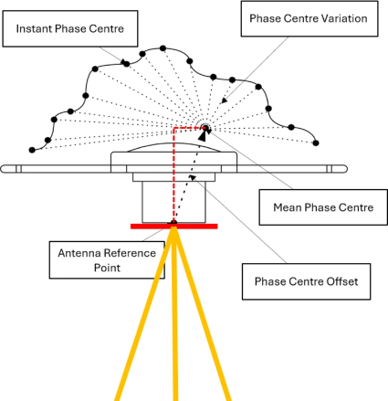
\includegraphics[width=0.35\linewidth]{images/pco_pcv.png}
    \caption{Schéma illustrant le décalage entre le point de référence d'une antenne et son centre de phase.}
    \label{fig:pco_pcv}
\end{figure}

\subsubsection{Phase Center Offset}

Le \textit{Phase Center Offset} correspond à un vecteur fixe, exprimé dans le
repère propre de l'antenne, reliant le point de référence de l'antenne à son
centre de phase. Ce décalage dépend notamment de la fréquence considérée et du
type d'antenne.

Pour l'antenne du récepteur, le PCO doit être projeté dans la direction
d'arrivée du signal afin de déterminer la contribution correspondante à la
distance mesurée. Pour l'antenne du satellite, le même principe s'applique en
tenant compte de l'orientation de l'antenne dans le repère du satellite.

Ainsi, si $\mathbf o_i$ désigne le vecteur PCO à la fréquence $i$ et
$\mathbf u_r^s$ le vecteur unitaire suivant la ligne de visée, la contribution
géométrique associée au PCO peut être exprimée sous la forme

\begin{align}
\Delta_{\mathrm{PCO},r,i}^s
=
\mathbf o_i\cdot\mathbf u_r^s,
\end{align}

le signe dépendant de la convention adoptée pour définir le vecteur de
visée et le PCO.

\subsubsection{Phase Center Variation}

Le centre de phase réel d'une antenne ne peut cependant pas être décrit par un
simple décalage constant. Sa position apparente varie avec la direction du
signal. Cette variation est appelée \textit{Phase Center Variation} (PCV).

La correction de PCV dépend généralement de l'angle d'élévation et, pour
certaines antennes, de l'azimut du signal. Elle est fournie sous forme de
modèles calibrés pour chaque type d'antenne et pour les différentes fréquences
GNSS.

Les informations nécessaires à la modélisation des PCO et PCV sont
généralement fournies dans les fichiers de calibration d'antennes au format
ANTEX. Ces fichiers permettent notamment d'associer à chaque modèle d'antenne
ses offsets de centre de phase ainsi que ses variations directionnelles pour
les différentes fréquences.

\subsubsection{Prise en compte dans le modèle d'observation}

Dans le cadre de ce projet, les corrections de centre de phase sont appliquées
aux antennes du satellite et du récepteur. La correction totale associée à une
observation peut ainsi être considérée comme la somme des contributions des
deux antennes :

\begin{align}
    \delta_{\mathrm{ant},r,i} = \Delta_{\mathrm{PCO},r,i} + \Delta_{\mathrm{PCV},r,i}
\end{align}

\begin{align}
    \delta_{\mathrm{ant},i}^{s} = \Delta_{\mathrm{PCO},i}^{s} + \Delta_{\mathrm{PCV},i}^{s}
\end{align}

Cette correction est calculée pour la fréquence et la direction de propagation
considérées. Dans le cas d'une combinaison ionosphère libre, les corrections
associées aux différentes fréquences sont elles-mêmes combinées avec les
mêmes coefficients que les observations correspondantes.

La prise en compte des centres de phase est particulièrement importante pour
un positionnement de précision. En effet, les décalages considérés sont
généralement de l'ordre du centimètre à plusieurs dizaines de centimètres et
peuvent donc devenir significatifs devant la précision recherchée.

\subsection{Enroulement de phase (\textit{wind-up})}\label{windup}

L'enroulement de phase (\textit{phase wind-up}) est un effet lié à la polarisation circulaire des signaux GNSS. Lorsque l'antenne d'émission du satellite tourne relativement à l'antenne de réception, la phase de la porteuse reçue varie d'un cycle complet pour chaque rotation de $360^\circ$. Cet effet n'affecte que les mesures de phase et peut s'accumuler sur plusieurs cycles au cours d'une session d'observation prolongée.

Les vecteurs d'antenne effectifs du satellite et du récepteur, projetés dans le plan perpendiculaire à la ligne de visée, s'écrivent

\begin{align}
\mathbf d^s
&=
\hat{\mathbf x}^s
-(\hat{\mathbf x}^s\cdot\hat{\mathbf k}_r^s)\hat{\mathbf k}_r^s
-\hat{\mathbf k}_r^s\times\hat{\mathbf y}^s,
\\
\mathbf d_r
&=
\hat{\mathbf x}_r
-(\hat{\mathbf x}_r\cdot\hat{\mathbf k}_r^s)\hat{\mathbf k}_r^s
+\hat{\mathbf k}_r^s\times\hat{\mathbf y}_r,
\end{align}

où

\begin{itemize}
    \item $\hat{\mathbf k}_r^s=-\mathbf u_r^s$ est le vecteur unitaire
    orienté du satellite $s$ vers le récepteur $r$, opposé au vecteur de visée ;
    \item $\hat{\mathbf x}^s$, $\hat{\mathbf y}^s$ sont les axes du repère propre de l'antenne du satellite ;
    \item $\hat{\mathbf x}_r$, $\hat{\mathbf y}_r$ sont les axes du repère propre de l'antenne du récepteur.
\end{itemize}

L'angle d'enroulement différentiel est donné par

\begin{align}
\cos\Delta\phi^s
=
\frac{\mathbf d^s\cdot\mathbf d_r}
{\|\mathbf d^s\|\,\|\mathbf d_r\|},
\end{align}

avec le signe déterminé par

\begin{align}
\operatorname{sign}(\Delta\phi^s)
=
\operatorname{sign}\!\left(
\hat{\mathbf k}_r^s\cdot(\mathbf d^s\times\mathbf d_r)
\right).
\end{align}

L'enroulement de phase s'accumule au cours du temps. La valeur cumulée $\phi_w^s(t)$ est mise à jour à chaque époque par

\begin{align}
\phi_w^s(t)
=
\phi_w^s(t-\Delta t)
+
\Delta\phi^s,
\end{align}

où $\Delta\phi^s$ est choisi tel que $|\Delta\phi^s|\leq\pi$ afin d'assurer la continuité de l'accumulation. La correction appliquée à la mesure de phase, exprimée en mètres, est alors

\begin{align}
\delta_{\mathrm{wind\text{-}up},r,i}^s
=
\lambda_i\,\phi_w^s(t),
\label{eq:windup}
\end{align}

où $\lambda_i$ est la longueur d'onde de la fréquence $i$. Pour un récepteur statique, l'orientation de l'antenne de réception est constante~: la variation de l'enroulement de phase est entièrement due à la rotation du satellite au cours de son orbite.

\subsection{Correction des marées terrestres}\label{marees}

Les marées terrestres solides sont des déformations périodiques de la croûte
terrestre induites principalement par les attractions gravitationnelles de la
Lune et du Soleil. Elles peuvent atteindre plusieurs dizaines de centimètres
en amplitude verticale. À la précision visée par le PPP, elles ne peuvent plus
être négligées.

Si $\Delta\mathbf{r}_{\mathrm{tide}}(t)$ désigne le déplacement du récepteur
sous l'effet des marées terrestres solides, la distance géométrique corrigée
s'écrit

\begin{align}
\rho_r^s(t)
=
\left\|
\mathbf{r}^s(t_e)
-\left(\mathbf{r}_r(t_r)
+\Delta\mathbf{r}_{\mathrm{tide}}(t_r)\right)
\right\|.
\label{eq:solid_tides_geometry}
\end{align}

Le déplacement $\Delta\mathbf{r}_{\mathrm{tide}}$ est calculé conformément
aux conventions de l'IERS (\textit{International Earth Rotation and Reference
Systems Service}), décrites dans les Conventions IERS 2010~\cite{iers2010}.
Dans l'implémentation retenue, ce calcul s'appuie sur les modèles fournis
par Orekit, qui appliquent les corrections de marées solides aux coordonnées
de la station.
